\section{Lecture 14: Discrete Time Fourier Transform }




%%%%%%%%%%%%%%%%%%%%%%%%%%%%%%%%%%%%%%%%%%%%%%%%%%%%%%%%%%%%%%%%%%%%%%%%%%%%


\subsection{Introduction}
We have so far talked about building a speech system, which would operate/process the signal in discrete time. For that, we first sample our periodic hence bandlimited signal, obeying the Nyquist principle. The resultant spectrum looks like this: (Specific signal chosen could have a different bandlimited spectrum than this, we've shown it to be linear just as an example)

\begin{figure}[htb]
\centering
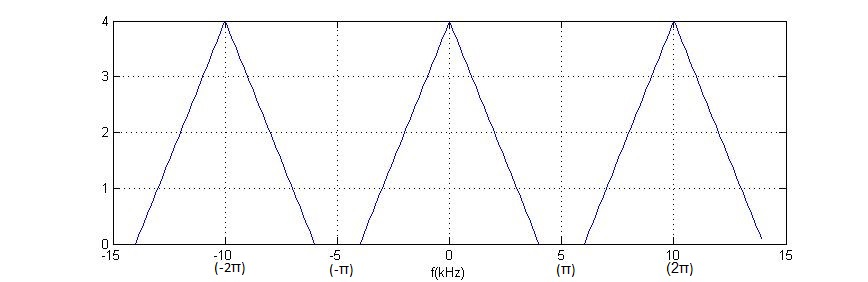
\includegraphics[width=0.7\textwidth]{spectrum.jpg}
\caption{\label{fig:spectrum}}
\end{figure}

Observe that the original spectrum exists here, along with its carbon copies or aliases. Now we change our x-axis to show normalized angular frequency, $\omega$ instead of cycles per second frequency as shown. In our example, the signal $x(t)$ is bandlimited by 4 kHz, and our sampling frequency is 10 kHz. So in the normalized angular frequency, 5 kHz will correspond to `$\pi$', 4 kHz to `$0.8\pi$' and so on, as shown.

\subsection{Discrete Time Fourier Transform}
Since we are processing the signal $x(t)$ in discrete time, our system along with signals can be represented as following:

\begin{figure}[htb]
\centering
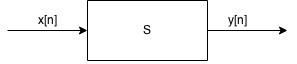
\includegraphics[width=0.4\textwidth]{sys.jpg}
\caption{}
\end{figure}

We'll choose our system to be the one described by $y[n]=\frac{x[n]+x[n-1]}{2}$. But for doing this, first we need to sample $x(t)$ to obtain x[n]. We have also decided to normalize our units, i.e choosing sampling interval as our unit of time, and sampling frequency as $f_s=1$ (for cycles/samples per second frequency) or $\Omega_s=2\pi$ (for angular frequency). In the chosen example, we have signal $x(t)$, which is a speech signal, sampled at 10 kHz i.e. taking 10,000 samples in each second. So our samples can be given as $x(nT_s)$, where $n\in\mathbb{Z}$ and $T_s = 0.1$ms.\\
So formally, the signal after sampling is given as 
\begin{align*}
\text{sampled signal}&=x(t)\sum\limits_{n=-\infty}^{+\infty} \delta(t-nT_s)\\
&=\sum\limits_{n=-\infty}^{+\infty} x(nT_s)\delta(t-nT_s)\\
\end{align*}
This is the signal which we'll give as input to the system $S$. Now the Fourier transform of our sampled signal will be
\begin{align*}
\text{FT of sampled signal}&=\int\limits_{-\infty}^{+\infty}\sum\limits_{n=-\infty}^{+\infty} x(nT_s)\delta(t-nT_s)e^{-j\Omega t}dt\\
\end{align*}
(If this integral converges, and we'd expect it to, for a speech signal, we'll exchange summation and integration) Hence
\begin{align*}
\text{FT of }x[n]&=\int\limits_{-\infty}^{+\infty}\sum\limits_{n=-\infty}^{+\infty} x(nT_s)\delta(t-nT_s)e^{-j\Omega t}dt\\
&=\sum\limits_{n=-\infty}^{+\infty}x(nT_s)\int\limits_{-\infty}^{+\infty}\delta(t-nT_s)e^{-j\Omega t}dt\\
&=\sum\limits_{n=-\infty}^{+\infty}x(nT_s)e^{-j\Omega nT_s}\\
\end{align*}
This, as we already know, represents the spectrum shown in this lecture. In terms of our normalization, we have,
\begin{align*}
x(nT_s)&=x[n]\\
\text{ also, }e^{-j\Omega nT_s}&=e^{-j\frac{\Omega}{\left(\frac{1}{T_s}\right)}n}\\
\text{But }\frac{\Omega}{\left(\frac{1}{T_s}\right)}&=\frac{2\pi\times\text{Actual cps frequency}}{\text{Sampling Frequency}}\\
&=\text{Normalized Angular Frequency, }\omega\\
\therefore e^{-j\Omega nT_s}&=e^{-j\omega n}\\
\end{align*}
\begin{align*}
\text{FT of sampled signal}&=\sum\limits_{n=-\infty}^{+\infty} x(nT_s)e^{-j\omega n}\\
&=\sum\limits_{n=-\infty}^{+\infty} x[n]e^{-j\omega n}\\
\end{align*}
This is essentially the Discrete Time Fourier Transform (DTFT) of $x(t)$ or of sequence $x[n]$. It is represented by $X(\omega)$. We can easily observe that it is essentially the component of $x[n]$ along $e^{j\omega n}$/inner product of $x[n]$ and  $e^{j\omega n}$. It tells us how much of $e^{j\omega n}$ is in the signal for each $n$.\\
As $\omega$ is the normalized angular frequency, spectrum of our signal would be upto $\omega=\pi$ strictly speaking. However, we shouldn't infact go upto $\omega=\pi$ and leave some margin as a buffer. For example, in the signal we have considered, $\omega=\pi$ corresponds to 5 kHz, but our signal only goes up to 4 kHz, or $\omega=0.8\pi$.
\subsection{Processing the Discretized Signal}

\begin{figure}[htb]
\centering
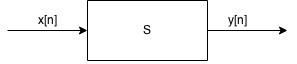
\includegraphics[width=0.4\textwidth]{sys.jpg}
\caption{}
\end{figure}

We had our system description as $y[n]=\frac{x[n]+x[n-1]}{2}$. Let us analyse what happens to a sinusoidal signal input. We are choosing sinusoid as we already know how to decompose a signal (if at all it is possible) in terms of sinusoids, and we have all the tools studied during our foray into Fourier domain analysis to help us. Speech signal, in particular, is usually bandlimited by 4 kHz, where lower frequencies are usually of the male voices (0-2 kHz) and female voices generally occupy higher frequencies (2-4 kHz). In our speech signal, we've considered a mixture of both male and female voices, as a general case. And we have sampled this signal at 10 kHz.\\
For analysis, we will use the rotating complex number representation of sinusoidal signal, $e^{j\omega n}$. So we have input to our system $x[n]=e^{j\omega n}$. And as $e^{j\omega n}$ is an eigen sequence, we know that a multiple of itself is going to come out as output, i.e. output will be of the form `$\text{constant}\times e^{j\omega n}$'. Using the system description we have,
\begin{align*}
y[n]&=\frac{x[n]+x[n-1]}{2}\\
&=\frac{e^{j\omega n}+e^{j\omega (n-1)}}{2}\\
&=\frac{1}{2}e^{j\omega n}\left(1+e^{-j\omega}\right)\\
\end{align*}
Hence the constant multiplying $e^{j\omega n}$ is $\frac{1}{2}\left(1+e^{-j\omega}\right)$. This constant can be simplified as:
\begin{align*}
\frac{1}{2}\left(1+e^{-j\omega}\right)&=\frac{1}{2}e^{-j\omega/2}(e^{j\omega/2}+e^{-j\omega/2})\\
&=\frac{1}{2}e^{-j\omega/2}(2\cos(\omega/2))\\
&=e^{-j\omega/2}\cos(\omega/2)
\end{align*}
In this form, we can easily identify the magnitude and phase factor, by which $e^{j\omega n}$ is multiplied. As magnitude of $e^{-j\omega/2}$ is one, it contributes only to the phase change, and as $\cos(\omega/2)$ corresponds to the magnitude change, and not to phase change, as in our range of $-\pi$ to $\pi$, $\cos(\omega/2)$ is a non-negative real number (hence has zero phase). This magnitude change can be plotted graphically in terms of $\omega$ as\\

\begin{figure}[htb]
\centering
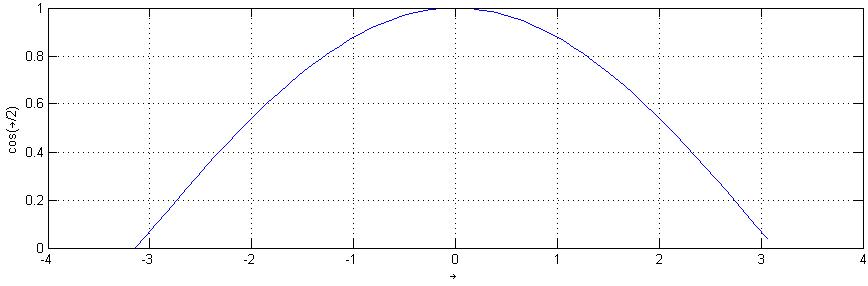
\includegraphics[width=0.7\textwidth]{cos.jpg}
\caption{}
\end{figure}

Remembering that 0-2 kHz represents predominantly the male voices, and 2-4 kHz the female voices, we see that this constant has higher magnitude for male voices, in general, than for the female voices. So this system enhances the male voices and suppresses the female voices.\\
The student is encouraged to try and find a simple system doing just the reverse thing, suppressing the male voices and enhancing the female voices. As a start, try considering $y[n]=\frac{x[n]-x[n-1]}{2}$, and giving it a rotating complex number as an input, $e^{j\omega n}$, to observe that the output is a multiple of this input, given by $\frac{e^{j\omega n}+e^{j\omega (n-1)}}{2}=\frac{1}{2}e^{j\omega n}\left(1+e^{-j\omega}\right)$. Analyse the constant to deduce that this system does the required job.

\subsection{Pondering About DTFT}
We observed that the DTFT of a signal is given by $X(\omega)=\sum\limits_{n=-\infty}^{\infty}x[n]e^{-j\omega n}$. We have confined $\omega$ within a region of length $\pi$. Let us try shifting this by $2\pi$:
\begin{align*}
X(\omega+2\pi)&=\sum\limits_{n=-\infty}^{\infty}x[n]e^{-j(\omega+2\pi) n}\\
&=\sum\limits_{n=-\infty}^{\infty}x[n]e^{-j\omega n}e^{-j2\pi n}\\
&=X(\omega)\text{  , as   }e^{-j2\pi n}=1\forall n
\end{align*}
Hence, shift of $2\pi$ make no difference, and this is what we'd expected, as DTFT is the spectrum of an ideally sampled signal, although written on normalized angular frequency axis. The spectrum of a discrete time sampled signal is always periodic, with a period of sampling frequency, and as we have normalized sampling frequency to $2\pi$, it is now periodic with $2\pi$. Also, any operations which we perform (as they are also in discrete time, with same time interval) are also periodic with the same interval of $2\pi$, and would act not only on the original spectrum, but also the carbon copies.\\
Also, we have done this analysis for signals sampled with ideal impulse-train sampling. A similar deed may be performed on signals sampled with pulse train sampling also, the case in which the carbon copies would have reduced magnitudes, but we'll not go there; however interested students are encouraged to try and think over it.




